% !TeX root = ../../main.tex
\chapter{Eksperymenty i rezultaty}

W niniejszym rozdziale przedstawione zostaną wyniki następujących eksperymentów:

\begin{itemize}
 \item Trening oryginalnej implementacji Mask R-CNN
 \item Trening zmodyfikowanej implemetacji Mask R-CNN z dokładniejszą maską
\end{itemize}

Wszystkie treningi korzystają z następującej strategii doboru parametru \textbf{learning\_rate}:

\TODO{explain}

Wyniki przedstawione w niniejszym rozdziale mogą zostać zreprodukowane z pomocą instrukcji~\footnote{\nameref{sec:instrukcja-instalacji}}~\footnote{\nameref{sec:instrukcja-uzytkownika}}.

\section{Zbiory danych}

Do przeprowadzenia eksperymentów użyto dwóch zbiorów danych, pozyskanych od firmy ``BLUE''. Jeden zbiór, zwany dalej zbiorem \textit{high} pochodzi z kamer ustawianych ponad kortem. Drugi zbiór, zwany dalej zbiorem \textit{low}, pochodzi z kamer sytuowanych na podłodze, tuż przy liniach kortu.

\begin{figure}[!htb]
  \minipage{0.45\textwidth}
    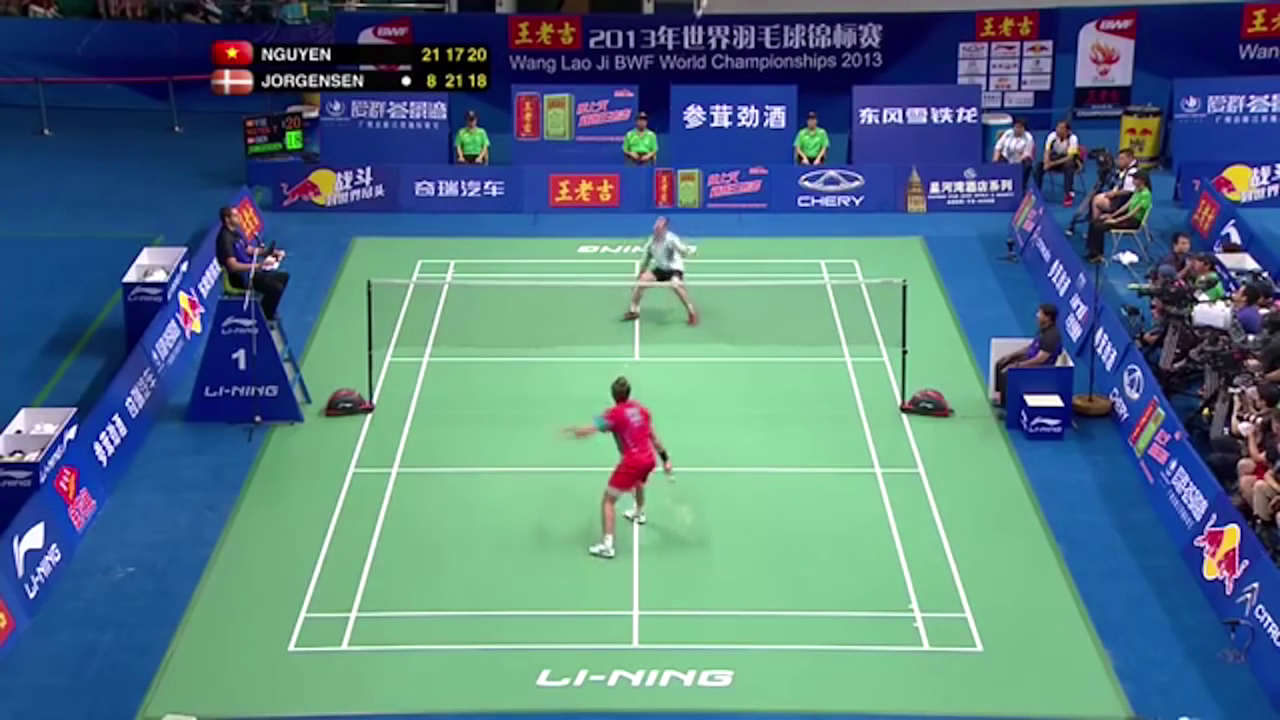
\includegraphics[width=\linewidth]{../badminton/datasets/badminton_high/train/test_court2-00002.png}
    \caption{Przykładowy obraz ze zbioru danych \textit{high}}
  \endminipage\hfill
  \minipage{0.45\textwidth}
    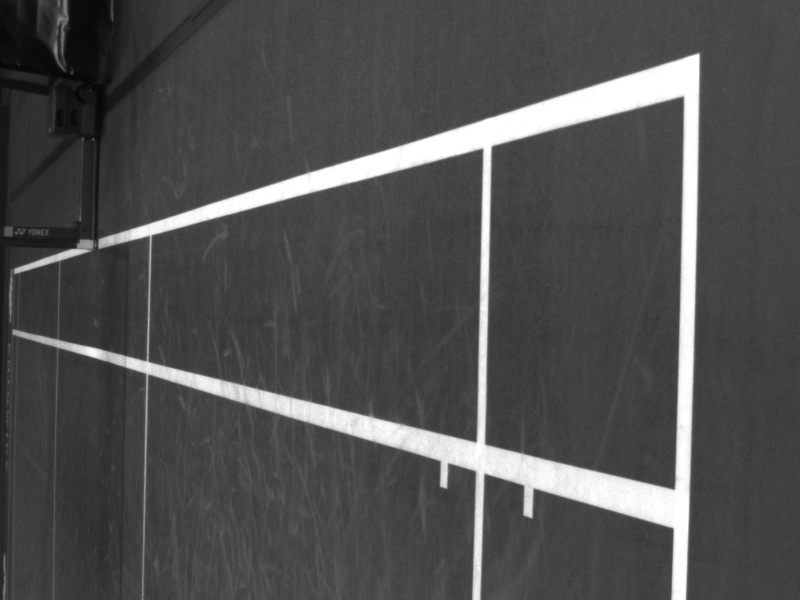
\includegraphics[width=\linewidth]{../badminton/datasets/badminton_low/train/1564909032792410075.jpg}
    \caption{Przykładowy obraz ze zbioru danych \textit{low}}
  \endminipage\hfill
  \end{figure}

\section{Wyniki z~użyciem sieci Mask R-CNN}

\begin{table}[!h]
	\centering
	\caption{Wyniki na zbiorze \textit{low}}
	\vspace{6pt}
	{\footnotesize
		\begin{tabular}{|c|c|c|c|c|}
			\hline \textbackslash & True Positive & False Positive & False Negative & True Negative \\
      \hline Worst & 2 (40\%) & 3 & 4 & 5 \\
      \hline Best & 2 & 3 & 4 & 5 \\
      \hline Median & 2 & 3 & 4 & 5 \\
      \hline Average & 2 & 3 & 4 & 5 \\
      \hline
		\end{tabular}
	}
	\vspace{0pt}
\end{table}

\vspace{1cm}

\begin{table}[!h]
	\centering
	\caption{Złożone wyniki \textit{low}}
	\vspace{6pt}
	{\footnotesize
		\begin{tabular}{|c|c|c|c|c|}
			\hline \textbackslash & Accuracy & Precision & Sensitivity & Specificity \\
      \hline Worst & 2 (40\%) & 3 & 4 & 5 \\
      \hline Best & 2 & 3 & 4 & 5 \\
      \hline Median & 2 & 3 & 4 & 5 \\
      \hline Average & 2 & 3 & 4 & 5 \\
      \hline
		\end{tabular}
	}
	\vspace{0pt}
\end{table}

\missingfigure{
  Tu będzie wykres rezultatów \textbf{niezmodyfikowanej} sieci Mask R-CNN \newline
  Oś X: Liczba epok treningowych \newline
  Oś Y: Poziom błędu na treningowym i na walidacyjnym  \newline
}

\missingfigure{Tu będzie screenshot ilustrujący problemu ``Falbanek''}

\section{Wyniki zmodyfikowanej sieci}
\label{sec:wyniki_zmodyfikowanej}

%loss - 0.01689
%val_loss = 0.03299
%val_mask_rcnn_loss = 0.01562

\missingfigure{
  Tu będzie wykres rezultatów \textbf{zmodyfikowanej} sieci Mask R-CNN \newline
  Na zbiorze \textbf{bez sztucznych danych}
}

\missingfigure{Tu będzie screenshot ilustrujący \textbf{rozwiązany} problem ``Falbanek''}

\section{Wyniki z~wykorzystaniem generatora}
\label{sec:wyniki_generator}

\missingfigure{
  Tu będzie wykres rezultatów zmodyfikowanej sieci Mask R-CNN \newline
  Na zbiorze \textbf{wzbogaconym o sztuczne dane}
}

\section{Rezultaty generalizacji zagadnienia}
\label{sec:generalizacja}

Praca skupia się na problemie detekcji kortu do badmintona, ale porusza też zagadnienie generalizacji rozwiązania na inne sporty z~kortem, jak na przykład tenis ziemny.
\\

\TODO{Tu będzie opis zgeneralizowania tytułowego problemu na tenis ziemny}

% // podsumowanie
% // tabela - podejscie, czas treningu do najlepszego rozwiazania, wynik val_mask_rcnn
